
% Default to the notebook output style

    


% Inherit from the specified cell style.




    
\documentclass{report}

    
    
    \usepackage{graphicx} % Used to insert images
    \usepackage{adjustbox} % Used to constrain images to a maximum size 
    \usepackage{color} % Allow colors to be defined
    \usepackage{enumerate} % Needed for markdown enumerations to work
    \usepackage{geometry} % Used to adjust the document margins
    \usepackage{amsmath} % Equations
    \usepackage{amssymb} % Equations
    \usepackage{eurosym} % defines \euro
    \usepackage[mathletters]{ucs} % Extended unicode (utf-8) support
    \usepackage[utf8x]{inputenc} % Allow utf-8 characters in the tex document
    \usepackage{fancyvrb} % verbatim replacement that allows latex
    \usepackage{grffile} % extends the file name processing of package graphics 
                         % to support a larger range 
    % The hyperref package gives us a pdf with properly built
    % internal navigation ('pdf bookmarks' for the table of contents,
    % internal cross-reference links, web links for URLs, etc.)
    \usepackage{hyperref}
    \usepackage{longtable} % longtable support required by pandoc >1.10
    \usepackage{booktabs}  % table support for pandoc > 1.12.2
    \usepackage{ulem} % ulem is needed to support strikethroughs (\sout)
    

    
    
    \definecolor{orange}{cmyk}{0,0.4,0.8,0.2}
    \definecolor{darkorange}{rgb}{.71,0.21,0.01}
    \definecolor{darkgreen}{rgb}{.12,.54,.11}
    \definecolor{myteal}{rgb}{.26, .44, .56}
    \definecolor{gray}{gray}{0.45}
    \definecolor{lightgray}{gray}{.95}
    \definecolor{mediumgray}{gray}{.8}
    \definecolor{inputbackground}{rgb}{.95, .95, .85}
    \definecolor{outputbackground}{rgb}{.95, .95, .95}
    \definecolor{traceback}{rgb}{1, .95, .95}
    % ansi colors
    \definecolor{red}{rgb}{.6,0,0}
    \definecolor{green}{rgb}{0,.65,0}
    \definecolor{brown}{rgb}{0.6,0.6,0}
    \definecolor{blue}{rgb}{0,.145,.698}
    \definecolor{purple}{rgb}{.698,.145,.698}
    \definecolor{cyan}{rgb}{0,.698,.698}
    \definecolor{lightgray}{gray}{0.5}
    
    % bright ansi colors
    \definecolor{darkgray}{gray}{0.25}
    \definecolor{lightred}{rgb}{1.0,0.39,0.28}
    \definecolor{lightgreen}{rgb}{0.48,0.99,0.0}
    \definecolor{lightblue}{rgb}{0.53,0.81,0.92}
    \definecolor{lightpurple}{rgb}{0.87,0.63,0.87}
    \definecolor{lightcyan}{rgb}{0.5,1.0,0.83}
    
    % commands and environments needed by pandoc snippets
    % extracted from the output of `pandoc -s`
    \providecommand{\tightlist}{%
      \setlength{\itemsep}{0pt}\setlength{\parskip}{0pt}}
    \DefineVerbatimEnvironment{Highlighting}{Verbatim}{commandchars=\\\{\}}
    % Add ',fontsize=\small' for more characters per line
    \newenvironment{Shaded}{}{}
    \newcommand{\KeywordTok}[1]{\textcolor[rgb]{0.00,0.44,0.13}{\textbf{{#1}}}}
    \newcommand{\DataTypeTok}[1]{\textcolor[rgb]{0.56,0.13,0.00}{{#1}}}
    \newcommand{\DecValTok}[1]{\textcolor[rgb]{0.25,0.63,0.44}{{#1}}}
    \newcommand{\BaseNTok}[1]{\textcolor[rgb]{0.25,0.63,0.44}{{#1}}}
    \newcommand{\FloatTok}[1]{\textcolor[rgb]{0.25,0.63,0.44}{{#1}}}
    \newcommand{\CharTok}[1]{\textcolor[rgb]{0.25,0.44,0.63}{{#1}}}
    \newcommand{\StringTok}[1]{\textcolor[rgb]{0.25,0.44,0.63}{{#1}}}
    \newcommand{\CommentTok}[1]{\textcolor[rgb]{0.38,0.63,0.69}{\textit{{#1}}}}
    \newcommand{\OtherTok}[1]{\textcolor[rgb]{0.00,0.44,0.13}{{#1}}}
    \newcommand{\AlertTok}[1]{\textcolor[rgb]{1.00,0.00,0.00}{\textbf{{#1}}}}
    \newcommand{\FunctionTok}[1]{\textcolor[rgb]{0.02,0.16,0.49}{{#1}}}
    \newcommand{\RegionMarkerTok}[1]{{#1}}
    \newcommand{\ErrorTok}[1]{\textcolor[rgb]{1.00,0.00,0.00}{\textbf{{#1}}}}
    \newcommand{\NormalTok}[1]{{#1}}
    
    % Additional commands for more recent versions of Pandoc
    \newcommand{\ConstantTok}[1]{\textcolor[rgb]{0.53,0.00,0.00}{{#1}}}
    \newcommand{\SpecialCharTok}[1]{\textcolor[rgb]{0.25,0.44,0.63}{{#1}}}
    \newcommand{\VerbatimStringTok}[1]{\textcolor[rgb]{0.25,0.44,0.63}{{#1}}}
    \newcommand{\SpecialStringTok}[1]{\textcolor[rgb]{0.73,0.40,0.53}{{#1}}}
    \newcommand{\ImportTok}[1]{{#1}}
    \newcommand{\DocumentationTok}[1]{\textcolor[rgb]{0.73,0.13,0.13}{\textit{{#1}}}}
    \newcommand{\AnnotationTok}[1]{\textcolor[rgb]{0.38,0.63,0.69}{\textbf{\textit{{#1}}}}}
    \newcommand{\CommentVarTok}[1]{\textcolor[rgb]{0.38,0.63,0.69}{\textbf{\textit{{#1}}}}}
    \newcommand{\VariableTok}[1]{\textcolor[rgb]{0.10,0.09,0.49}{{#1}}}
    \newcommand{\ControlFlowTok}[1]{\textcolor[rgb]{0.00,0.44,0.13}{\textbf{{#1}}}}
    \newcommand{\OperatorTok}[1]{\textcolor[rgb]{0.40,0.40,0.40}{{#1}}}
    \newcommand{\BuiltInTok}[1]{{#1}}
    \newcommand{\ExtensionTok}[1]{{#1}}
    \newcommand{\PreprocessorTok}[1]{\textcolor[rgb]{0.74,0.48,0.00}{{#1}}}
    \newcommand{\AttributeTok}[1]{\textcolor[rgb]{0.49,0.56,0.16}{{#1}}}
    \newcommand{\InformationTok}[1]{\textcolor[rgb]{0.38,0.63,0.69}{\textbf{\textit{{#1}}}}}
    \newcommand{\WarningTok}[1]{\textcolor[rgb]{0.38,0.63,0.69}{\textbf{\textit{{#1}}}}}
    
    
    % Define a nice break command that doesn't care if a line doesn't already
    % exist.
    \def\br{\hspace*{\fill} \\* }
    % Math Jax compatability definitions
    \def\gt{>}
    \def\lt{<}
    % Document parameters
    \title{Jak-na-Git}
    
    
    

    % Pygments definitions
    
\makeatletter
\def\PY@reset{\let\PY@it=\relax \let\PY@bf=\relax%
    \let\PY@ul=\relax \let\PY@tc=\relax%
    \let\PY@bc=\relax \let\PY@ff=\relax}
\def\PY@tok#1{\csname PY@tok@#1\endcsname}
\def\PY@toks#1+{\ifx\relax#1\empty\else%
    \PY@tok{#1}\expandafter\PY@toks\fi}
\def\PY@do#1{\PY@bc{\PY@tc{\PY@ul{%
    \PY@it{\PY@bf{\PY@ff{#1}}}}}}}
\def\PY#1#2{\PY@reset\PY@toks#1+\relax+\PY@do{#2}}

\expandafter\def\csname PY@tok@sd\endcsname{\let\PY@it=\textit\def\PY@tc##1{\textcolor[rgb]{0.73,0.13,0.13}{##1}}}
\expandafter\def\csname PY@tok@kd\endcsname{\let\PY@bf=\textbf\def\PY@tc##1{\textcolor[rgb]{0.00,0.50,0.00}{##1}}}
\expandafter\def\csname PY@tok@mi\endcsname{\def\PY@tc##1{\textcolor[rgb]{0.40,0.40,0.40}{##1}}}
\expandafter\def\csname PY@tok@c\endcsname{\let\PY@it=\textit\def\PY@tc##1{\textcolor[rgb]{0.25,0.50,0.50}{##1}}}
\expandafter\def\csname PY@tok@gd\endcsname{\def\PY@tc##1{\textcolor[rgb]{0.63,0.00,0.00}{##1}}}
\expandafter\def\csname PY@tok@nf\endcsname{\def\PY@tc##1{\textcolor[rgb]{0.00,0.00,1.00}{##1}}}
\expandafter\def\csname PY@tok@nv\endcsname{\def\PY@tc##1{\textcolor[rgb]{0.10,0.09,0.49}{##1}}}
\expandafter\def\csname PY@tok@ss\endcsname{\def\PY@tc##1{\textcolor[rgb]{0.10,0.09,0.49}{##1}}}
\expandafter\def\csname PY@tok@cm\endcsname{\let\PY@it=\textit\def\PY@tc##1{\textcolor[rgb]{0.25,0.50,0.50}{##1}}}
\expandafter\def\csname PY@tok@w\endcsname{\def\PY@tc##1{\textcolor[rgb]{0.73,0.73,0.73}{##1}}}
\expandafter\def\csname PY@tok@cpf\endcsname{\let\PY@it=\textit\def\PY@tc##1{\textcolor[rgb]{0.25,0.50,0.50}{##1}}}
\expandafter\def\csname PY@tok@gs\endcsname{\let\PY@bf=\textbf}
\expandafter\def\csname PY@tok@nb\endcsname{\def\PY@tc##1{\textcolor[rgb]{0.00,0.50,0.00}{##1}}}
\expandafter\def\csname PY@tok@cp\endcsname{\def\PY@tc##1{\textcolor[rgb]{0.74,0.48,0.00}{##1}}}
\expandafter\def\csname PY@tok@ch\endcsname{\let\PY@it=\textit\def\PY@tc##1{\textcolor[rgb]{0.25,0.50,0.50}{##1}}}
\expandafter\def\csname PY@tok@na\endcsname{\def\PY@tc##1{\textcolor[rgb]{0.49,0.56,0.16}{##1}}}
\expandafter\def\csname PY@tok@s\endcsname{\def\PY@tc##1{\textcolor[rgb]{0.73,0.13,0.13}{##1}}}
\expandafter\def\csname PY@tok@vc\endcsname{\def\PY@tc##1{\textcolor[rgb]{0.10,0.09,0.49}{##1}}}
\expandafter\def\csname PY@tok@gt\endcsname{\def\PY@tc##1{\textcolor[rgb]{0.00,0.27,0.87}{##1}}}
\expandafter\def\csname PY@tok@sr\endcsname{\def\PY@tc##1{\textcolor[rgb]{0.73,0.40,0.53}{##1}}}
\expandafter\def\csname PY@tok@kp\endcsname{\def\PY@tc##1{\textcolor[rgb]{0.00,0.50,0.00}{##1}}}
\expandafter\def\csname PY@tok@mo\endcsname{\def\PY@tc##1{\textcolor[rgb]{0.40,0.40,0.40}{##1}}}
\expandafter\def\csname PY@tok@s2\endcsname{\def\PY@tc##1{\textcolor[rgb]{0.73,0.13,0.13}{##1}}}
\expandafter\def\csname PY@tok@sh\endcsname{\def\PY@tc##1{\textcolor[rgb]{0.73,0.13,0.13}{##1}}}
\expandafter\def\csname PY@tok@vg\endcsname{\def\PY@tc##1{\textcolor[rgb]{0.10,0.09,0.49}{##1}}}
\expandafter\def\csname PY@tok@k\endcsname{\let\PY@bf=\textbf\def\PY@tc##1{\textcolor[rgb]{0.00,0.50,0.00}{##1}}}
\expandafter\def\csname PY@tok@kn\endcsname{\let\PY@bf=\textbf\def\PY@tc##1{\textcolor[rgb]{0.00,0.50,0.00}{##1}}}
\expandafter\def\csname PY@tok@il\endcsname{\def\PY@tc##1{\textcolor[rgb]{0.40,0.40,0.40}{##1}}}
\expandafter\def\csname PY@tok@gr\endcsname{\def\PY@tc##1{\textcolor[rgb]{1.00,0.00,0.00}{##1}}}
\expandafter\def\csname PY@tok@nc\endcsname{\let\PY@bf=\textbf\def\PY@tc##1{\textcolor[rgb]{0.00,0.00,1.00}{##1}}}
\expandafter\def\csname PY@tok@ni\endcsname{\let\PY@bf=\textbf\def\PY@tc##1{\textcolor[rgb]{0.60,0.60,0.60}{##1}}}
\expandafter\def\csname PY@tok@nn\endcsname{\let\PY@bf=\textbf\def\PY@tc##1{\textcolor[rgb]{0.00,0.00,1.00}{##1}}}
\expandafter\def\csname PY@tok@err\endcsname{\def\PY@bc##1{\setlength{\fboxsep}{0pt}\fcolorbox[rgb]{1.00,0.00,0.00}{1,1,1}{\strut ##1}}}
\expandafter\def\csname PY@tok@nt\endcsname{\let\PY@bf=\textbf\def\PY@tc##1{\textcolor[rgb]{0.00,0.50,0.00}{##1}}}
\expandafter\def\csname PY@tok@sb\endcsname{\def\PY@tc##1{\textcolor[rgb]{0.73,0.13,0.13}{##1}}}
\expandafter\def\csname PY@tok@vi\endcsname{\def\PY@tc##1{\textcolor[rgb]{0.10,0.09,0.49}{##1}}}
\expandafter\def\csname PY@tok@o\endcsname{\def\PY@tc##1{\textcolor[rgb]{0.40,0.40,0.40}{##1}}}
\expandafter\def\csname PY@tok@kr\endcsname{\let\PY@bf=\textbf\def\PY@tc##1{\textcolor[rgb]{0.00,0.50,0.00}{##1}}}
\expandafter\def\csname PY@tok@ne\endcsname{\let\PY@bf=\textbf\def\PY@tc##1{\textcolor[rgb]{0.82,0.25,0.23}{##1}}}
\expandafter\def\csname PY@tok@gp\endcsname{\let\PY@bf=\textbf\def\PY@tc##1{\textcolor[rgb]{0.00,0.00,0.50}{##1}}}
\expandafter\def\csname PY@tok@nd\endcsname{\def\PY@tc##1{\textcolor[rgb]{0.67,0.13,1.00}{##1}}}
\expandafter\def\csname PY@tok@go\endcsname{\def\PY@tc##1{\textcolor[rgb]{0.53,0.53,0.53}{##1}}}
\expandafter\def\csname PY@tok@nl\endcsname{\def\PY@tc##1{\textcolor[rgb]{0.63,0.63,0.00}{##1}}}
\expandafter\def\csname PY@tok@gi\endcsname{\def\PY@tc##1{\textcolor[rgb]{0.00,0.63,0.00}{##1}}}
\expandafter\def\csname PY@tok@mf\endcsname{\def\PY@tc##1{\textcolor[rgb]{0.40,0.40,0.40}{##1}}}
\expandafter\def\csname PY@tok@ow\endcsname{\let\PY@bf=\textbf\def\PY@tc##1{\textcolor[rgb]{0.67,0.13,1.00}{##1}}}
\expandafter\def\csname PY@tok@cs\endcsname{\let\PY@it=\textit\def\PY@tc##1{\textcolor[rgb]{0.25,0.50,0.50}{##1}}}
\expandafter\def\csname PY@tok@se\endcsname{\let\PY@bf=\textbf\def\PY@tc##1{\textcolor[rgb]{0.73,0.40,0.13}{##1}}}
\expandafter\def\csname PY@tok@mh\endcsname{\def\PY@tc##1{\textcolor[rgb]{0.40,0.40,0.40}{##1}}}
\expandafter\def\csname PY@tok@gu\endcsname{\let\PY@bf=\textbf\def\PY@tc##1{\textcolor[rgb]{0.50,0.00,0.50}{##1}}}
\expandafter\def\csname PY@tok@si\endcsname{\let\PY@bf=\textbf\def\PY@tc##1{\textcolor[rgb]{0.73,0.40,0.53}{##1}}}
\expandafter\def\csname PY@tok@kt\endcsname{\def\PY@tc##1{\textcolor[rgb]{0.69,0.00,0.25}{##1}}}
\expandafter\def\csname PY@tok@m\endcsname{\def\PY@tc##1{\textcolor[rgb]{0.40,0.40,0.40}{##1}}}
\expandafter\def\csname PY@tok@no\endcsname{\def\PY@tc##1{\textcolor[rgb]{0.53,0.00,0.00}{##1}}}
\expandafter\def\csname PY@tok@kc\endcsname{\let\PY@bf=\textbf\def\PY@tc##1{\textcolor[rgb]{0.00,0.50,0.00}{##1}}}
\expandafter\def\csname PY@tok@gh\endcsname{\let\PY@bf=\textbf\def\PY@tc##1{\textcolor[rgb]{0.00,0.00,0.50}{##1}}}
\expandafter\def\csname PY@tok@bp\endcsname{\def\PY@tc##1{\textcolor[rgb]{0.00,0.50,0.00}{##1}}}
\expandafter\def\csname PY@tok@ge\endcsname{\let\PY@it=\textit}
\expandafter\def\csname PY@tok@c1\endcsname{\let\PY@it=\textit\def\PY@tc##1{\textcolor[rgb]{0.25,0.50,0.50}{##1}}}
\expandafter\def\csname PY@tok@sx\endcsname{\def\PY@tc##1{\textcolor[rgb]{0.00,0.50,0.00}{##1}}}
\expandafter\def\csname PY@tok@sc\endcsname{\def\PY@tc##1{\textcolor[rgb]{0.73,0.13,0.13}{##1}}}
\expandafter\def\csname PY@tok@mb\endcsname{\def\PY@tc##1{\textcolor[rgb]{0.40,0.40,0.40}{##1}}}
\expandafter\def\csname PY@tok@s1\endcsname{\def\PY@tc##1{\textcolor[rgb]{0.73,0.13,0.13}{##1}}}

\def\PYZbs{\char`\\}
\def\PYZus{\char`\_}
\def\PYZob{\char`\{}
\def\PYZcb{\char`\}}
\def\PYZca{\char`\^}
\def\PYZam{\char`\&}
\def\PYZlt{\char`\<}
\def\PYZgt{\char`\>}
\def\PYZsh{\char`\#}
\def\PYZpc{\char`\%}
\def\PYZdl{\char`\$}
\def\PYZhy{\char`\-}
\def\PYZsq{\char`\'}
\def\PYZdq{\char`\"}
\def\PYZti{\char`\~}
% for compatibility with earlier versions
\def\PYZat{@}
\def\PYZlb{[}
\def\PYZrb{]}
\makeatother


    % Exact colors from NB
    \definecolor{incolor}{rgb}{0.0, 0.0, 0.5}
    \definecolor{outcolor}{rgb}{0.545, 0.0, 0.0}



    
    % Prevent overflowing lines due to hard-to-break entities
    \sloppy 
    % Setup hyperref package
    \hypersetup{
      breaklinks=true,  % so long urls are correctly broken across lines
      colorlinks=true,
      urlcolor=blue,
      linkcolor=darkorange,
      citecolor=darkgreen,
      }
    % Slightly bigger margins than the latex defaults
    
    \geometry{verbose,tmargin=1in,bmargin=1in,lmargin=1in,rmargin=1in}
    
    

    \begin{document}
    
    
    %\maketitle
    
    

    
    \chapter*{Jak na GIT}\label{jak-na-git}

    \begin{quote}
\textbf{Git} je distribuovaný systém správy verzí vytvořený Linusem
Torvaldsem, původně pro vývoj jádra Linuxu.
\end{quote}

    Pokud vám na téhle větě není něco jasného, zeptejte se hned, nebo se
podívejte přímo na stránky
\href{https://cs.wikipedia.org/wiki/Git}{Wikipedie}, ze které tento
citát pochází. Jako první krok v seznamování se s Gitem by bylo víc než
vhodné navštívit jeho webovou prezentaci na adrese
\textbf{\url{https://git-scm.com/}}. Právě tam naleznete instrukce, jak
Git bezplatně a legálně získat i rady jak jej nainstalovat pod svým
operačním systémem. Pro rychlé seznámení jsou v rámci obsáhlé
dokumentace k dispozici i krátké instruktážní videa, či on-line trenažér
pro okamžité vyzkoušení.

    \begin{figure}[htbp]
\centering
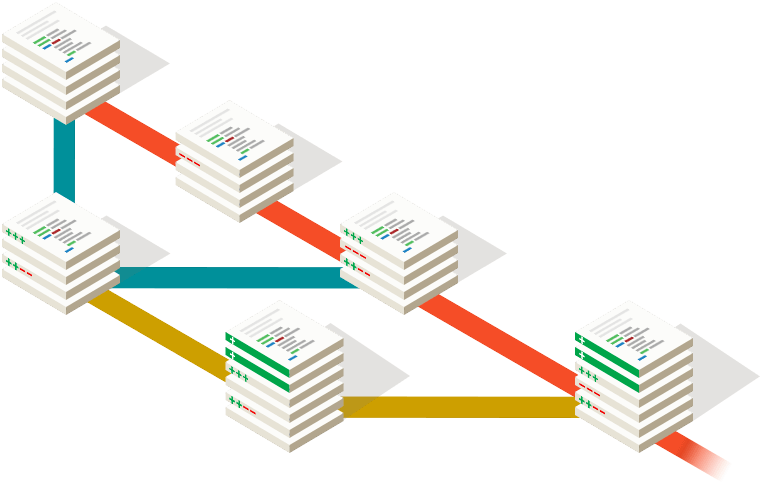
\includegraphics[width=\linewidth]{../images/branching-illustration@2x.png}
\caption{Branching illustration}
\end{figure}

    \section*{Verzování}\label{verzovuxe1nuxed}

Takový vývoj, jak už název sám naznačuje je dynamický proces, při němž
nezávislí jedinci z celého světa tvořící otevřenou komunitu postupně
upravují určité dokumenty. Ať už se jedná o zdrojové kódy numerických
simulací, pomocné skripty pro grafickou prezentaci výsledků, podklady
pro inovativní článek v prestižním vědeckém časopise, nebo jen
interaktivní webovou prezentaci pro praktický tutoriál na konferenci.
Aby z toho nebyl úplný chaos, je třeba jejich práci efektivně řídit. A
právě k tomu účelu se víc než skvěle hodí systém pro správu verzí. A
protože ve verzích bývá často guláš, je dobré vědět s jakou konkrétní
verzi daného programu právě pracujeme.

\begin{Shaded}
\begin{Highlighting}[]
\NormalTok{$ }\KeywordTok{git} \NormalTok{--version}
\KeywordTok{git} \NormalTok{version 2.7.0}
\end{Highlighting}
\end{Shaded}

V zájmu reprodukovatelnosti vědeckého bádání je proto vhodné uvádět i
čísla verzí programového vybavení použitého při vývoji numerických
simulací i pro dodatečnou analýzu jejich výsledků. Pro usnadnění tohoto
procesu připravil \emph{Robert Johansson}, autor unikátního studijního
materiálu
\href{https://github.com/jrjohansson/scientific-python-lectures}{\textbf{Lectures
on scientific computing with Python}}, rozšíření pro Jupyter notebook
\texttt{\%version\_information}. To lze pohodlně nainstalovat
standardním postupem

\begin{Shaded}
\begin{Highlighting}[]
\NormalTok{$ }\KeywordTok{pip} \NormalTok{install version_information}
\end{Highlighting}
\end{Shaded}

Jeho použití v Jupyter notebooku je pak záležitostí jen dvou magických
příkazů, které by se měly objevit dle libosti buď na začátku, nebo na
konci každého notebooku.

    \begin{Verbatim}[commandchars=\\\{\}]
{\color{incolor}In [{\color{incolor}1}]:} \PY{o}{\PYZpc{}}\PY{k}{load\PYZus{}ext} version\PYZus{}information
        \PY{o}{\PYZpc{}}\PY{k}{version\PYZus{}information} numpy, scipy, matplotlib
\end{Verbatim}
\texttt{\color{outcolor}Out[{\color{outcolor}1}]:}
    
    \begin{tabular}{|l|l|}\hline
{\bf Software} & {\bf Version} \\ \hline\hline
Python & 3.5.1 64bit [GCC 5.2.0] \\ \hline
IPython & 4.0.1 \\ \hline
OS & Linux 4.3.3 3 ARCH x86\_64 with arch \\ \hline
numpy & 1.10.4 \\ \hline
scipy & 0.16.1 \\ \hline
matplotlib & 1.5.1 \\ \hline
\hline \multicolumn{2}{|l|}{Wed Jan 20 11:33:55 2016 CET} \\ \hline
\end{tabular}

    

    \section*{Nápověda}\label{nuxe1povux11bda}

Tak jako většina slušně napsanýc programů, ani \texttt{git} není
vyjímkou v přijímání přepínače \texttt{-\/-help}, který zaručí vypsání
stručné nápovědy ohledně jeho použití. Více detailů o chování
jednotlivých příkazů se dočtete v přehledné dokumentaci pčímo na webu
nebo ve formě manuálových stránek, které zběhlý uživatel některé z
distribuce operačního systému GNU/Linux jistě dobře zná.

\begin{Shaded}
\begin{Highlighting}[]
\NormalTok{$ }\KeywordTok{git} \NormalTok{--help}

\KeywordTok{usage}\NormalTok{: git [--version] [--help] [-C }\KeywordTok{<}\NormalTok{path}\KeywordTok{>}\NormalTok{] [-c name=value]}
           \NormalTok{[}\KeywordTok{--exec-path}\NormalTok{[=}\KeywordTok{<}\NormalTok{path}\KeywordTok{>}\NormalTok{]] [--html-path] [--man-path] [--info-path]}
           \NormalTok{[}\KeywordTok{-p} \KeywordTok{|} \KeywordTok{--paginate} \KeywordTok{|} \KeywordTok{--no-pager}\NormalTok{] [--no-replace-objects] [--bare]}
           \NormalTok{[}\KeywordTok{--git-dir}\NormalTok{=}\KeywordTok{<}\NormalTok{path}\KeywordTok{>}\NormalTok{] [--work-tree=}\KeywordTok{<}\NormalTok{path}\KeywordTok{>}\NormalTok{] [--namespace=}\KeywordTok{<}\NormalTok{name}\KeywordTok{>}\NormalTok{]}
           \KeywordTok{<command>} \NormalTok{[}\KeywordTok{<}\NormalTok{args}\KeywordTok{>}\NormalTok{]}

\KeywordTok{These} \NormalTok{are common Git commands used in various situations:}

\KeywordTok{start} \NormalTok{a working area (see also: git help tutorial)}
   \KeywordTok{clone}      \NormalTok{Clone a repository into a new directory}
   \KeywordTok{init}       \NormalTok{Create an empty Git repository or reinitialize an existing one}

\KeywordTok{work} \NormalTok{on the current change (see also: git help everyday)}
   \KeywordTok{add}        \NormalTok{Add file contents to the index}
   \KeywordTok{mv}         \NormalTok{Move or rename a file, a directory, or a symlink}
   \KeywordTok{reset}      \NormalTok{Reset current HEAD to the specified state}
   \KeywordTok{rm}         \NormalTok{Remove files from the working tree and from the index}

\KeywordTok{examine} \NormalTok{the history and state (see also: git help revisions)}
   \KeywordTok{bisect}     \NormalTok{Use binary search to find the commit that introduced a bug}
   \KeywordTok{grep}       \NormalTok{Print lines matching a pattern}
   \KeywordTok{log}        \NormalTok{Show commit logs}
   \KeywordTok{show}       \NormalTok{Show various types of objects}
   \KeywordTok{status}     \NormalTok{Show the working tree status}

\KeywordTok{grow}\NormalTok{, mark and tweak your common history}
   \KeywordTok{branch}     \NormalTok{List, create, or delete branches}
   \KeywordTok{checkout}   \NormalTok{Switch branches or restore working tree files}
   \KeywordTok{commit}     \NormalTok{Record changes to the repository}
   \KeywordTok{diff}       \NormalTok{Show changes between commits, commit and working tree, etc}
   \KeywordTok{merge}      \NormalTok{Join two or more development histories together}
   \KeywordTok{rebase}     \NormalTok{Forward-port local commits to the updated upstream head}
   \KeywordTok{tag}        \NormalTok{Create, list, delete or verify a tag object signed with GPG}

\KeywordTok{collaborate} \NormalTok{(see also: git help workflows)}
   \KeywordTok{fetch}      \NormalTok{Download objects and refs from another repository}
   \KeywordTok{pull}       \NormalTok{Fetch from and integrate with another repository or a local branch}
   \KeywordTok{push}       \NormalTok{Update remote refs along with associated objects}

\StringTok{'git help -a'} \KeywordTok{and} \StringTok{'git help -g'} \NormalTok{list available subcommands and some}
\KeywordTok{concept} \NormalTok{guides. See }\StringTok{'git help <command>'} \NormalTok{or }\StringTok{'git help <concept>'}
\KeywordTok{to} \NormalTok{read about a specific subcommand or concept.}
\end{Highlighting}
\end{Shaded}

Samozřejmě nechybí ani automatické doplňování argumentů příkazu v
příkazové řádce okna terminálu po opakovaném stisku klávesy
\texttt{\textless{}Tab\textgreater{}}. I zde stejně jako i jinde platí,
že v případě výskytu nějaké chyby, dříve než začnete propadat panice, si
napřed v klidu přečtěte, co se \texttt{git}u nelíbí a pokud jste
rozumní, poslechněte i jeho rady ohledně toho, co dělat dál

\begin{Shaded}
\begin{Highlighting}[]
\NormalTok{$ }\KeywordTok{git} \NormalTok{tak}

\KeywordTok{git}\NormalTok{: }\StringTok{'tak'} \NormalTok{is not a git command. See }\StringTok{'git --help'}\NormalTok{.}

\KeywordTok{Did} \NormalTok{you mean this?}
    \KeywordTok{tag}
\end{Highlighting}
\end{Shaded}

    \section*{Nastavení}\label{nastavenuxed}

První věcí, kterou byste pro úspěšné použití \texttt{git}u měli udělat,
je vyplnění svých kontaktních údajů, podle nichž budou moci býti
identifikovány všechny vaše příspěvky napříč virtuálními komunitami a to
až do konce existence Internetu. Jedině tak vaše dobré skutky budou moci
býti po zásluze odměněny.

\begin{Shaded}
\begin{Highlighting}[]
\NormalTok{$ }\KeywordTok{git} \NormalTok{config --global user.name }\StringTok{"John Doe"}
\NormalTok{$ }\KeywordTok{git} \NormalTok{config --global user.email johndoe@example.com}
\end{Highlighting}
\end{Shaded}

Pro efektivnější používání \texttt{git}u z příkazové řádky terminálu,
kterému se budete dále věnovat převážně sami ať už během volných nocí
při dohledu nad automatickým teleskopem či vesmírnou družicí, je
užitečné nastavit přinejmenším svůj oblíbený textový editor, ve kterém
rádi píšete.

\begin{Shaded}
\begin{Highlighting}[]
\NormalTok{$ }\KeywordTok{git} \NormalTok{config --global core.editor nano}
\end{Highlighting}
\end{Shaded}

Nyní již nastal čas vytvořit si svůj první \emph{repozitář}. To je
místo, ideálně někde v \emph{cloudu}, kde budou vaše dokumenty bezpečně
a zároveň přístupně uloženy včetně historie jejich změn, ať už se na
nich podílel kdokoliv. To je totiž přesně to, co \texttt{git} dělá.
Ukládá historii změn dokumentů. A tím tajemným místem je
\textbf{GitHub}. Momentálně asi nejpopulárnější ze sociálních sítí
zaměřených na sdílení zdrojových kódů průběžně vyvíjených programů.
Navíc tam můžete s dalšími kolegy debatovat nad společně tvořeným dílem
v příjemném prostředí moderní webové aplikace. Ať už z pohodlí křesla
vaší kanceláře, gauče zadního salóku ve vaší oblíbené kavárně, nebo jen
v jídelním voze rychlíku mířícího z nejzapadlejšího koutu Republiky do
právě budovaného Centra Excelence.

    \section*{Repozitář}\label{repozituxe1ux159}

Nový projekt můžete začít různými způsoby. Tím nejsnažším je kliknutí na
ikonu \href{https://github.com/new}{\textbf{+}} hnedle vedle vašeho
avataru na stránce GitHubu. Ovšem to jen za předpokladu, že jste jeho
registrovanými uživateli a jste-li přihlášení ke svému účtu. Pak už jen
stačí následovat přímočaré instrukce, které vám ponouká. Další možností,
pokud nechcete začínat vyloženě od nuly, je tak zvané \emph{forknutí}
již existujícího repozitáře, i na to najdete příslušné tlačítko přímo na
stránce daného repozitáře. Pak už jen stačí, si vybraný repozitář
\emph{naklonovat}, což ač to zní kdo ví jak děsivě, je jen jiný výraz
pro stažení\ldots{}

\begin{Shaded}
\begin{Highlighting}[]
\NormalTok{$ }\KeywordTok{git} \NormalTok{clone https://github.com/}\KeywordTok{<}\NormalTok{GITHUBNAME}\KeywordTok{>}\NormalTok{/astro123.git}
\end{Highlighting}
\end{Shaded}

Pokud chcete již stažený repozitář aktualizovat, použijte příkaz

\begin{Shaded}
\begin{Highlighting}[]
\NormalTok{$ }\KeywordTok{git} \NormalTok{pull}
\end{Highlighting}
\end{Shaded}

Tím jste právě získali svou vlastní a aktuální kopii. Co s ní budete dál
dělat je už jen na vás. Pokud se ale rozhodnete řešit přiložené úlohy,
což je i jednou z nutných podmínek k získání zápočtu a připuštění ke
zkoušce, může vám být ku prospěchu pár dobře míněných rad.

    \subsection*{Větvení}\label{vux11btvenuxed}

Nejen že \texttt{git} umožňuje cestování do minulosti, ale zároveň je
možné se s ním pohybovat i v paralerním prostoru, těm se říká
\emph{větve} a představa košatého stromu je tady zcela oprávněná. Novou
větev pojmenovanu ideálně podle svého uča vytvoříte příkazem

\begin{Shaded}
\begin{Highlighting}[]
\NormalTok{$ }\KeywordTok{git} \NormalTok{branch 123456}
\end{Highlighting}
\end{Shaded}

Přejít do ní můžete za pomoci příkazu

\begin{Shaded}
\begin{Highlighting}[]
\NormalTok{$ }\KeywordTok{git} \NormalTok{checkout 123456}
\end{Highlighting}
\end{Shaded}

Všechny změny, které od této chvíle provedete se dějí v oddělené větvi
mimo tu hlavní zvanou \emph{master}. A tak by to mělo být pokaždé, když
plánujete do již fungujícího konceptu zavést novou změnu, že si napřed
vytvoříte svou vlastní pracovní kopii, se kterou dále nakládáte podle
svého vlastního uvážení, jak nejrozumněji umíte.

    \subsection*{Příspěvky}\label{pux159uxedspux11bvky}

Nyní již můžete do správy verzovacího systému \texttt{git} přidat soubor
s řešením, který jste sami vytvořili.

\begin{Shaded}
\begin{Highlighting}[]
\NormalTok{$ }\KeywordTok{git} \NormalTok{add solutions/}\KeywordTok{<}\NormalTok{UČO}\KeywordTok{>}\NormalTok{-}\KeywordTok{<}\NormalTok{Jméno}\KeywordTok{>}\NormalTok{+}\KeywordTok{<}\NormalTok{Příjmení}\KeywordTok{>}\NormalTok{_Úloha.ipynb}
\end{Highlighting}
\end{Shaded}

O aktuálním stavu repozitáře, se můžete přesvědčit příkazem

\begin{Shaded}
\begin{Highlighting}[]
\NormalTok{$ }\KeywordTok{git} \NormalTok{status}
\end{Highlighting}
\end{Shaded}

a neméně užitečný je i příkaz pro zobrazení historických záznamů

\begin{Shaded}
\begin{Highlighting}[]
\NormalTok{$ }\KeywordTok{git} \NormalTok{log}
\end{Highlighting}
\end{Shaded}

Teď nastal čas připrav příspěvek se stručnou zprávou, která se odešlě
spolu s provedenými změnami. Ten pište tak, jako kdyby jste někomu
posílal e-mail s přílohou. Myslete při tom na to, že ho bude číst
nejenom vaše budoucí \emph{já}, ale potenciálně i někdo bez spětky
smyslu pro humor, cynizmu či nadsázky, tak se prosím snažtě, ať alespoň
trochu dává smysl.

\begin{Shaded}
\begin{Highlighting}[]
\NormalTok{$ }\KeywordTok{git} \NormalTok{commit}
\end{Highlighting}
\end{Shaded}

Nyní už jen stačí odeslat příspěvek do vzdáleného repozitáře.

\begin{Shaded}
\begin{Highlighting}[]
\NormalTok{$ }\KeywordTok{git} \NormalTok{push origin 123456}
\end{Highlighting}
\end{Shaded}

Na závěr, zpátky na webové stránce vašeho repozitáře na GitHubu,
vytvořte požadavek na přetažení do originálního repozitáře. A trpělivě
vyčkejte reakce od jeho správce. Mějte přitom na paměti, že tem může být
z naprosto jiného časového pásma než vy, tak na něj zbytečně
nenaléhejte, pokud to není vyloženě nutné.

Pokud jste se dostali až sem, tak vám blahopřeji. Právě jste zvládli
ovládnout technologii, která vám umožní podílet se na zajímavých
projektech ve společnosti celoplanetárního vědeckého týmu.

    \section*{Odměna}\label{odmux11bna}

Pro vášnivého čtenáře si dovolim doporučit i jednu knihu, na takové to
domácí čtení při dlouhých zimních večerech. Dostupná je i v českém
překladu a elektronickou verzi si můžete stáhnout zdarma z edice knih
správce České národní domény \href{https://knihy.nic.cz/}{CZ.NIC}.

\begin{quote}
 \textbf{Pro Git}. \emph{Scott Chacon} je popularizátorem systému správy
verzí Git a pracuje také jako vývojář v Ruby na projektu GitHub.com Git
je distribuovaný systém pro správu verzí, který se používá zejména při
vývoji svobodného a open source softwaru. Git si klade za cíl být
rychlým a efektivním nástrojem pro správu verzí. V knize se čtenář
seznámí jak se stát rychlým a efektivním při jeho používání. Seznámí se
nejen s principy používání, ale také s detaily jak Git funguje interně
nebo s možnostmi, které nabízejí některé další doplňkové nástroje.
\end{quote}


    % Add a bibliography block to the postdoc
    
    
    
    \end{document}
